\chapter{Diseño e implementación}

En este capítulo se describirán las clases y todos los métodos que se han añadido y modificado durante el proceso de implementación a partir del código base de OpenBabel en su versión 3.1.1 (disponible en su repositorio oficial de GitHub\footnote{\url{https://github.com/openbabel/openbabel/releases}}). OpenBabel está escrito en C++, por lo que el proceso de desarrollo se ha llevado a cabo exclusivamente en este lenguaje, usando para ello el IDE \textit{Visual Studio C++} para Windows, (en el Anexo \ref{apend:manual} se detalla este proceso).


\section{Diseño}

\subsection{Estructura de OpenBabel}

A partir del código fuente de OpenBabel, al compilar los archivos fuente y generar el proyecto, los archivos de configuración de CMake generan una serie de \emph{soluciones}. Hay soluciones que consisten únicamente en el archivo `\textit{main}', que representa el ejecutable al que llamamos por línea de órdenes desde la terminal. El resto de soluciones forman la propia API de OpenBabel, siendo las clases más importantes `OBMol', `OBAtom', y `OBBond', que permiten almacenar la información de una molécula, un átomo, o un enlace entre átomos respectivamente; y otras clases más orientadas a la conversión entre formatos como `OBConversion' u `OBFormat'.

A continuación se muestra la estructura general de directorios de OpenBabel:
\vspace{0.5cm}
\dirtree{%
.1 openbabel-3-1-1/.
    .2 cmake/\DTcomment{\textit{algunos ficheros de configuración para cmake}}.
    .2 data/\DTcomment{}.
    .2 doc/\DTcomment{\textit{documentación del proyecto y ficheros para su generación automática}}.
    .2 include/\DTcomment{\textit{ficheros .h}}.
        .3 openbabel/.
            .4 depict/\DTcomment{\textit{representación de moléculas}}.
            .4 math/.
            .4 stereo/.
            .4 tree/.
            .4 clases principales de Openbabel.
                .5 ....
    .2 src/\DTcomment{\textit{ficheros .cpp}}.
        .3 charges/.
        .3 depict/\DTcomment{\textit{representación de moléculas}}.
        .3 descriptors/.
        .3 fingerprints/.
        .3 formats/\DTcomment{\textit{soporte para distintos formatos de conversión}}.
        .3 math/.
        .3 ops/\DTcomment{\textit{plugins de la comunidad}}.
        .3 stereo/.
        .3 clases principales de Openbabel.
            .4 ....
    .2 scripts/\DTcomment{\textit{bindings para usar la interfaz en otros lenguajes}}.
    .2 test/\DTcomment{\textit{ficheros de ejecución de tests y datos de prueba}}.
    .2 tools/\DTcomment{\textit{\textit{'mains'} para ejecución por línea de órdenes}}.
    .2 CMakeLists.txt\DTcomment{\textit{archivo principal de configuración de cmake}}.
    .2 INSTALL\DTcomment{\textit{instrucciones breves de instalación de openbabel}}.
    .2 ficheros propios de .git\DTcomment{}.
}


\subsection{Diagrama de Clases}

 En el siguiente Diagrama de clases (Figura \ref{fig:diagrama_clases}) se muestran tanto las clases que se han visto modificadas (en color anaranjado), las creadas desde cero (en color más verdoso) y las demás clases importantes que interactúan con las anteriores pero no se han visto alteradas (en amarillo). 

\begin{landscape}

    \begin{figure}[]
        \centering
        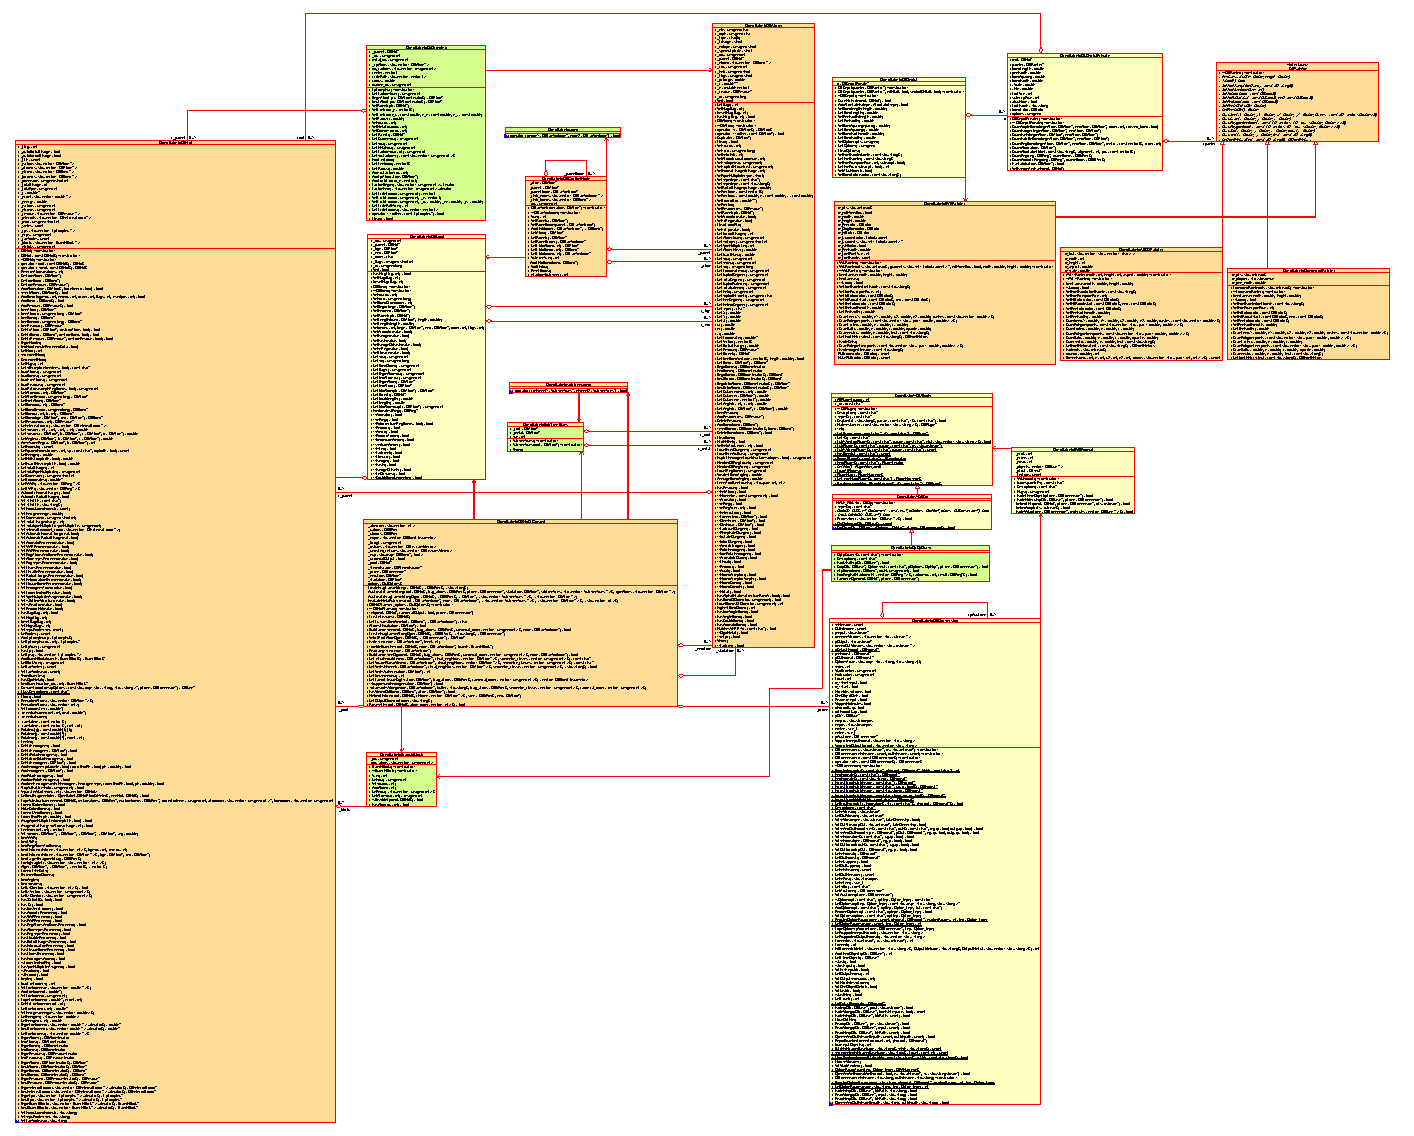
\includegraphics[scale=0.7]{imagenes/diseno/diagramaClasesHorizontal_cropped.pdf}
        \caption{Diagrama de clases}
        \label{fig:diagrama_clases}
    \end{figure}
\end{landscape}

% 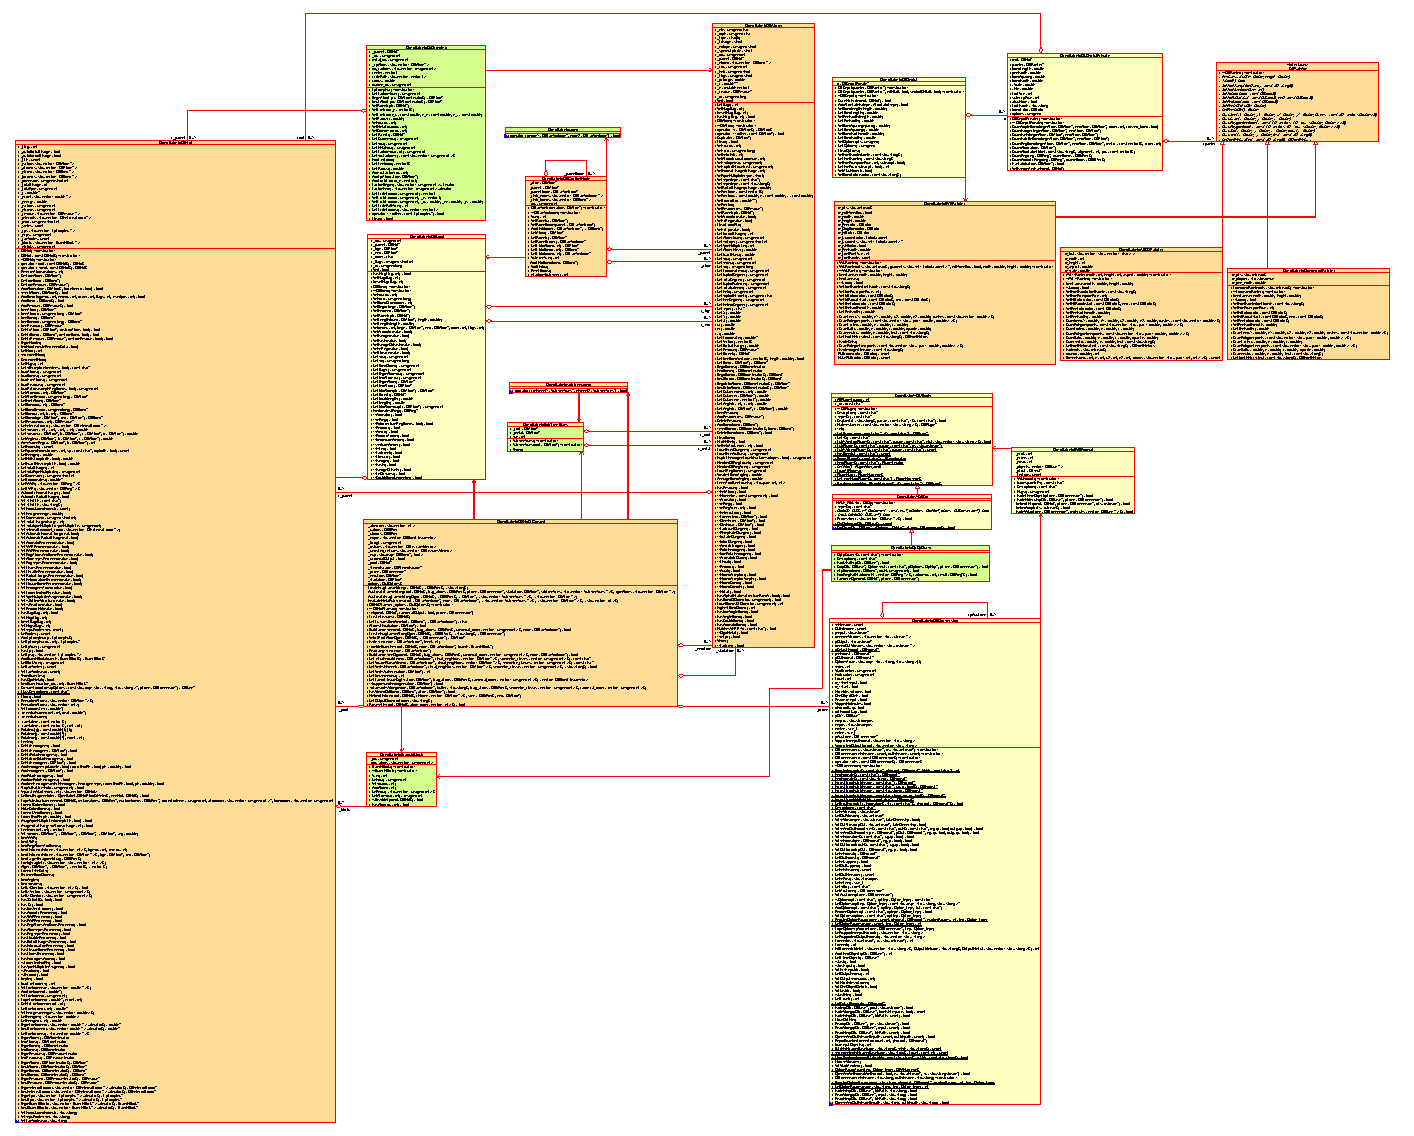
\includepdf[pages=-, offset=0 0,landscape=true,]{imagenes/diseno/diagramaClasesHorizontal_cropped.pdf}


Se pasa a detallar ahora cada una de las clases, tanto las modificadas como las nuevas, para qué sirven, y en qué consisten sus métodos. Las clases que no se han alterado, al igual que el resto de clases que no se incluyen en el diagrama se puede consultar su documentación en la página oficial\footnotemark. Puntualizar que existe una enorme cantidad de clases en la librería de OpenBabel, no tendería sentido añadirlas todas en el diagrama. Además, no todas poseen de documentación, por lo que la mayoría no aparecerán en\footnote[1]{\url{https://openbabel.github.io/api/3.0/index.shtml}}.


%  ------------------------- Cabeceras -------------------------
\subsection{Clases modificadas}
\begin{itemize}
    \item \textbf{OBPainter}: clase base abstracta para las clases de representación gráfica 2D (en \textit{/depict/painter.h}). Se ha añadido el siguiente método para poder utilizarlo en las clases que implementan esta interfaz:
    \begin{lstlisting}[language=C++]
        public: 
    
virtual void DrawPolygonLine(const std::vector<std::pair<double, double> >& points) = 0;
    \end{lstlisting}

    \item \textbf{SVGPainter}: clase que hereda de OBPainter y genera representaciones 2D en el formato de gráficos vectoriales SVG (en \textit{/depict/svgpainter.h}).
    \begin{lstlisting}[language=C++]
        public: 
    
//Inserts the necessary xml code in the .svg output file to draw a polygon according to the vector of points specified by @p points
void DrawPolygonLine(const std::vector<std::pair<double, double> >& points);
    \end{lstlisting}

    \item \textbf{ASCIIPainter}: clase que hereda de OBPainter (en \textit{/depict/asciipainter.h}).
    \begin{lstlisting}[language=C++]
        public: 
    
//The method is declared empty to avoid compilation errors due to interface implementation. It has no use 
void DrawPolygonLine(const std::vector<std::pair<double, double> >& points);
    \end{lstlisting}

    \item \textbf{CommandPainter}: clase que hereda de OBPainter (en \textit{/depict/commandpainter.h}).
    \begin{lstlisting}[language=C++]
        public: 
    
//The method is declared empty to avoid compilation errors due to interface implementation. It has no use 
void DrawPolygonLine(const std::vector<std::pair<double, double> >& points);
    \end{lstlisting}

    % -------------------------- Atom ---------------------------
    \item \textbf{OBAtom}: clase principal, contiene la información relativa a un átomo, guardando su número atómico, cantidad de hidrógenos implícitos, una lista de los enlaces de este átomo con los demás y el vector de coordenadas 2D para su representación, entre otras variables (en \textit{/openbabel/atom.h}). Se han añadido los siguientes métodos:
    \begin{lstlisting}[language=C++]
class OBAPI OBAtom: public OBBase{
    public: 
    
//\return Is this a metal commonnly present in organometallic compounds?
bool IsOgmMetal();

//\return Is atom part of a Cp ring?
bool IsInCp() const;

//\return Is this atom a Carbon (atomic number == 6)?
bool IsCarbon();

//Debug method. Displays on basic output simple data to identify the atom
void Show();

//Mark an atom as part of a Cp ring
void SetInCp(bool value = true);
};//class
    \end{lstlisting}


    % -------------------------- Mol ---------------------------
    \item \textbf{OBMol}: clase principal, almacena toda la información básica relacionada con una molécula. Esto incluye la lista de átomos, la lista completa de enlaces entre átomos, identificadores de los átomos y enlaces, y el vector de coordenadas 2D de todos los átomos para su representación entre otras variables (en \textit{/openbabel/mol.h}). Se han añadido las siguientes variables y métodos:
    \begin{lstlisting}[language=C++]
class OBAPI OBMol: public OBBase {
    private: 
    
std::string _smiles;                //!< Input smiles string for the molecule
std::vector<CpComplex*> _cps;       //!< Cp information
unsigned int _ncps;                 //!< Number of cps complexes detected
std::string  _canSmiles;            //!< Canonical smiles based on Ogm canonicalization
std::vector<BranchBlock*> _blocks;  //!< Branches information
unsigned int _nblocks;              //!< Number of blocks


    public: 
    
//! Set the input smiles string of this molecule to @p smi
void SetInputSmiles(std::string smi);

//! \return the input smiles string of this molecule
std::string GetSmiles();

//! Add a new CpComplex specified by @p cp
void AddCpComplex(CpComplex& cp);

//! \return the cp at index @p idx or NULL if none exists.
CpComplex* GetCpComplex(int idx);

//! \return number of cp in the molecule
unsigned int GetCpSize();

//! \return whether the molecule has cps or not
bool HasCp();

//! \return the whole container of cps of this molecule
std::vector<CpComplex*> GetCps();

//! Add a new block to the molecule, specified by @p branch
BranchBlock* AddBranchBlock(BranchBlock& branch);

//! \return the number of blocks in the molecule
unsigned int GetBlockSize();

//! \return the canonical smiles string generated by the ogm canonicalization methods
std::string GetCanSmiles();

//! Set the canonical smiles string of this molecule to @p smi
void   SetCanSmiles(std::string smi);

//! Debug method. Displays on basic output all molecule blocks with basic information of the atoms.
void ShowBranches();

//! \return If this molecule has any Ogm metal or not
bool HasOgmMetal();

//! \return the block of which the carbon at index @p carbon_idx is part, or NULL if no such block exists
BranchBlock* FindBranch(int carbon_idx);

//! Set the iterator to the beginning of the Cp list
//! \return the first Cp structure, or NULL if none exist
CpComplex* BeginCp(std::vector<CpComplex*>::iterator & i);

//! Advance the iterator to the next Cp record
//! \return the next first Cp record, or NULL if none exist
CpComplex* NextCp(std::vector<CpComplex*>::iterator& i);

//! Set the iterator to the beginning of the BranchBlock list
//! \return the first BranchBlock structure, or NULL if none exist
BranchBlock* BeginBranchBlock(std::vector<BranchBlock*>::iterator& i);

//! Advance the iterator to the next BranchBlock record
//! \return the next first BranchBlock record, or NULL if none exist
BranchBlock* NextBranchBlock(std::vector<BranchBlock*>::iterator& i);
};//class
    \end{lstlisting}


    % -------------------------- OBMol2Cansmi ---------------------------
    \item \textbf{OBMol2Cansmi}: clase que maneja la conversión del smiles de entrada a un smiles canónico (en \textit{src/formats/smilesformat.h}). Se han añadido los siguientes métodos:
    \begin{lstlisting}[language=C++]
class OBMol2Cansmi{}
        private: 
    
//Only changed visibility to private, since CreateFragCansmiStringOgm was created. Selects the "root" atom, which will be first in the SMILES, then builds a tree in canonical order, and finally generates the SMILES.
void CreateFragCansmiString(OBMol&, OBBitVec&, std::string&);

    
//Auxiliary private methods for SelectRootAtomOgm

//Shortened version of the CreateCansmiString method. Create the necessary variables to call AuxCreateFragCansmiStringOgm.
void AuxCreateCansmiString(OBMol& mol, OBBitVec& frag_atoms, OBConversion* pConv, OBAtom* startatom, std::vector<SubTreeSizes*>& subtreeSizes, std::vector<OBAtom*> ogmAtoms);

//Shortened version of the CreateFragCansmiStringOgm method. Create the necessary variables to build a new canonical tree using as root @p startAtom
void AuxCreateFragCansmiStringOgm(OBMol&, OBBitVec&, OBAtom*, std::vector<SubTreeSizes*>&, std::vector<OBAtom*>);

//Once the tree is built, this method runs through it in DFS evaluating the subtrees hanging from the other ogm metals. Use the auxiliary struct SubTreeSizes for this. 
void EvaluateMetalSubTrees(OBCanSmiNode* root, OBCanSmiNode* node, std::vector<SubTreeSizes*>&, std::vector<OBAtom*>&, std::vector<int>&);

        public: 
//Method based on CreateFragCansmiString. Share much of the code, with some additional methods specifically for my own canonical form designed for organometallic molecules.
void CreateFragCansmiStringOgm(OBMol&, OBBitVec&, std::string&, OBConversion*);

//If more than 1 Ogm metal is present in the molecule, this method chooses one of them, based on some rules and the conectivity of the metal within the molecule and the rest of the atoms
OBAtom* SelectRootAtomOgm(OBMol&, OBConversion*);

//Debug method for writing in basic output the tree with hierarchy formating
void WriteTree(OBCanSmiNode* node, int level = 0);

//Adds information to the molecule of the blocks that form it. Being a block, each set of atoms that, due to their bonds, are within the same parenthesis in the original input Smiles. Or, according to the OBMol2Cansmi::BuildCanonTree method, the parent-child relationship between atoms.
void IdentifyBranches(OBMol& mol,OBCanSmiNode* node, BranchBlock* branch = nullptr);

//Modifies the tree built by BuildCanonTree based on the length of the branches identified in IdentifyBranches. This is a canonical rule designed for a little more consistency in the output canon smiles.
void RearrangeTree(OBCanSmiNode* node);

//Builds the SMILES tree, in canonical order, for the specified molecular fragment. Based on the BuildCanonTree method. Shares much of the code, with some changes in the neighbour selection algorithm.
bool BuildCanonTreeOgm(OBMol& mol, OBBitVec& frag_atoms, vector<unsigned int>& canonical_order, OBCanSmiNode* node);
};//class
    \end{lstlisting}


    % -------------------------- OBCanSmiNode ---------------------------
    \item \textbf{OBCanSmiNode}: clase que representa un nodo. En conjunto se forma una estructura de árbol, cada nodo es un átomo del árbol para luego escribir el SMILES canónico (en \textit{src/formats/smilesformat.h}). Se han añadido los elementos:
    \begin{lstlisting}[language=C++]
class OBMol2Cansmi{
        private: 
    
OBCanSmiNode* _parentNode;      //!< Pointer to the parent node

//! Add a child bond to the node, specified by @p bond. Should only be used in the ResetBonds method as a part of the OBMol2Cansmi::RearrangeTree algorithm.
//! Otherwise, use addChildnode to add both the child node and its respective bonds
void AddChildBond(OBBond* bond);

        public: 

//! Set the parent node to @p parent
void SetParentNode(OBCanSmiNode* parent);

//! \return the parent node
OBCanSmiNode* GetParentNode();

//! Traverses the tree in dfs from the node calling the method
//! \return the number of total children (counting himself) 
int SubTreeSize();

//! Sort a node's child_nodes using a std::sort operation an a custom comparator 'mycomp'
void SortChilds();

//! When added at the same time in the addchildnode method, the child with its bond have a 1 to 1 index correspondence. When reordering the children, in OBMol2Cansmi::RearrangeTree, the indices of the bonds are lost. This method clears and adds the bonds back in order.
void ResetBonds();

//! \return the total number of carbons in this node subtree
int nCarbonsSubTree();
};//class
    \end{lstlisting}

\end{itemize}





\subsection{Clases nuevas}
\begin{itemize}
    % -------------------------- CpComplex ---------------------------
    \item \textbf{CpComplex}: nueva clase principal que maneja y permite almacenar estructuras de ciclopentadienilo (en \textit{/openbabel/cpcomplex.h}). Se han creado las siguientes variables y métodos:
    \begin{lstlisting}[language=C++]
class CpComplex {
	protected:
  
OBMol* _parent;                         //!< Parent molecule
unsigned int _idx;                      //!< Cp identifier within the molecule
unsigned int metal_idx;                 //!< Atom idx of central metal
std::vector<OBAtom*> _cpAtoms;          //!< Atoms for the carbons of the Cp structure
std::vector<unsigned int> idx_carbons;  //!< Atom indexes for the carbons of the Cp structure
vector3 center;                         //!< Cp center, for normal bond connection with metal atom, and aromatic circle position
std::vector<vector3> circlePath;        //!< Coordinates for the cp circle (needed to achieve a perspective circunference)
double radius;                          //!< Cp's aromatic circle radius
unsigned int dummy_idx;                 //!< Dummy central atom idx


        public:

//! Default constructor 
CpComplex();

//! \name Methods to modify internal information
//@{
//! Attach an OBMol @p ptr as the parent container for this Cp
void SetParent(OBMol* ptr);
//! Set the center point of the Cp, sprecified by @p _v. It is equidistant to every carbon in th Cp, as they are disposed in a regular polygon
void SetCentroid(vector3& _v);
//! Set the center point of the Cp, sprecified by @p v_x, v_y, v_z. It is equidistant to every carbon in th Cp, as they are disposed in a regular polygon
void SetCentroid(const double v_x, const double v_y, const double v_z);
//! Set the radius of the Cp circle
void SetRadius(double r);
//! Set the Cp identifier
void SetIdx(int idx);
//! Set the idx of the central metal to which this Cp is attached
void SetMetalIdx(int midx);
//! Dummy atom is created to make a perpendicular bond between the metal and the Cp drawing
//! Set the atom idx of the dummy atom created for this Cp 
void SetDummyIdx(int idx);
//! Set the point of the Cp circle at index @p i to the coordinates specified by @p _v
void SetCircleCoord(unsigned int i, vector3 _v);
//! Set the point of the Cp circle at index @p i to the coordinates specified by @p _vx, _vy, _vz
void SetCircleCoord(unsigned int i, double _vx, double _vy, double _vz = 0.0);
//@}


//! \name Methods to retrieve information
//@{
//! \return number of carbon atoms in the cp
unsigned int GetCarbonsSize();
//! \return the molecule which contains this Cp, or NULL if none exists
OBMol* GetParent();
//! \return dummy atom idx for this Cp structure, or 0 if none exists
unsigned int GetDummyIdx() const;
//! \return Cp identifier
unsigned int GetIdx() const;
//! \return Central metal identifier
unsigned int GetMetalIdx() const;
//! \return carbon idx at position @p i in tha container. Zero based access method to vector
unsigned int GetCarbonIdx(int i) const;
//! \return the whole contanier of carbon idx
const std::vector<unsigned int>& GetIdxCarbons();
//! \return the centroid of this Cp in a coordinate vector
vector3& GetCentroid();
//! \return the radius of the Cp circle
double GetRadius();
//! \return the coordinate vector for the Cp circle point at position @p i in the container. Zero based access method to vector
vector3 GetCircleCoord(unsigned int i);
//! \return the number of points of the Cp circle
int GetCirclePathSize() const;
//! \return the whole container of coordinates of the Cp circle
std::vector<vector3> GetCircleCoords() const;
//@}


//! \name Addition of data for a Cp
//@{
//! Adds a new atom idx to this Cp
void AddIdxCarbon(int idx);
//! Adds a new atom to this Cp
void AddCpAtom(OBAtom* atom);
//! Adds a new point to the coordinate vector that forms the Cp circle
void AddCircleCoord(vector3 _v);
//@}


//! \name Iteration methods
//@{
//! Set the iterator to the beginning of the Cp atom list
//! \return the first atom, or NULL if none exist
OBAtom* CpComplex::BeginAtomCp(OBAtomIterator& i);
//! Advance the iterator to the next atom in the Cp
//! \return the next first atom record, or NULL if none exist
OBAtom* CpComplex::NextAtomCp(OBAtomIterator& i);
//@}


//! \name Other operations
//@{
//! Calculate and set the centroid of this Cp, taking into consideration all atoms stored in _cpAtoms
void FindCentroid();
//! Equivalence operator
bool operator==(const CpComplex* other) const;
//@}
};//class
    \end{lstlisting}


    % -------------------------- BranchBlock ---------------------------
    \item \textbf{BranchBlock}: clase que representa un grupo funcional aislado dentro de la molécula, p.ej. un ciclo de benceno, un Cp, o toda una rama de un átomo (en \textit{/openbabel/cpcomplex.h}). Se han añadido las siguientes variables y métodos:
    \begin{lstlisting}[language=C++]
class BranchBlock {
        private: 
    
unsigned int _idx;                          //!< Block identifier
std::vector<unsigned int> vidx_atoms;       //!< Vector idx of the atoms that are part of the block.

        public: 

//! Default constructor
BranchBlock();

//! Destructor
~BranchBlock();

//! \return the size of the block (number of atoms in the block)
int Size();

//! \return the block identifier
unsigned int GetIdx();

//! Set the block identifier
void SetIdx(int idx);

//! Add an atom's idx to the block
void AddAtom(int i);

//! \return the idx of the atom at position @p i. Zero based access.
unsigned int GetAtomIdx(int i);

//! \return Whether the @p idx exists within the atoms already inserted in the block
bool HasAtom(int idx);

//! Cp will be possible if all the elements in the block are carbons up to that point and have a bond with an ogm metal.
//! \return whether or not it appears to be a Cp block
bool IsPossibleCp(OBMol &mol)
}; //class
    \end{lstlisting}


    % -------------------------- OpCpDraw ---------------------------
    \item \textbf{OpCpDraw}: clase plugin que hereda de OBOp (en \textit{/ops/cpdraw.cpp}). Contiene el algoritmo de detección, identificación, y almacenamiento en la molécula de estructuras tipo Cp.
    \begin{lstlisting}[language=C++]
class class OpCpDraw : public OBOp {
//! Default constructor
OpCpDraw(const char* ID);

//! Inherited method. 
//! Display through the output stream a brief description of the plugin.
const char* Description();

//! Inherited method. 
//! \return true if this op (plugin operation) is designed to work with the class of @p pOb, e.g. OBMol
virtual bool WorksWith(OBBase* pOb) const;

//! Inherited method. Required function that does the work. Normally return true, unless object is not to be output. 
virtual bool Do(OBBase* pOb, const char* OptionText = nullptr, OpMap* pOptions = nullptr, OBConversion* pConv = nullptr);

//! \return If @p bond is likely to be a cp-bond like
bool isCpBond(OBBond* bond, unsigned int idxM);

//! Finds the ring of which the carbon with idx @p carbonIdx is a part of, among the rings of @p rlist (obtained from a SSSR perspective), and stores it in @p result.
//! \returns whether it was found or not
bool FindRingWithCarbon(vector<OBRing*>& rlist, int carbonIdx, OBRing*& result);

//! Canonize the input SMILES and identify blocks
void CanonizeOgm(OBMol* mol, OBConversion* pConv); 
}; //class
    \end{lstlisting}


    
    % -------------------------- SubTreeSizes ---------------------------
    \item \textbf{SubTreeSizes}: struct auxiliar creado para la selección del primer metal durante la canonización (se profundiza sobre esto en la Sección \ref{canonizacion}). Contiene las siguientes variables y métodos (en \textit{src/formats/smilesformat.h}):
    \begin{lstlisting}[language=C++]
struct SubTreeSizes {

OBAtom* _root;      //!< Tree root
OBAtom* _metal;     //!< Metal to evaluate
int size;           //!< Size of the subtree for the _metal to evaluate
int nCarbons;       //!< Number of carbon atoms

//! Default constructor
SubTreeSizes();

//! Parameter constructor. Creates a new object with _root as @p root
SubTreeSizes(OBAtom* root);

//! Debug method. Displays through basic output the struct information.
void Show();
};//struct
    \end{lstlisting}


    % -------------------------- subtreecomp ---------------------------
    \item \textbf{subtreecomp}: objeto comparador que prioriza unos metales sobre otros en el proceso de selección del átomo raíz para el árbol (en \textit{src/formats/smilesformat.h}).
    \begin{lstlisting}[language=C++]
struct subtreecomp {
bool operator() (SubTreeSizes* element1, SubTreeSizes* element2) const;
}subtreecomp;
    \end{lstlisting}


    % -------------------------- mycomp ---------------------------
    \item \textbf{mycomp}: objeto comparador que prioriza las ramas del árbol canónico durante el proceso de reordenación (en \textit{src/formats/smilesformat.h}).
    \begin{lstlisting}[language=C++]
struct comp{
bool operator() (OBCanSmiNode* node1, OBCanSmiNode* node2);
}mycomp;
    \end{lstlisting}
    
\end{itemize}


En resumen, se han modificado 8 clases existentes, sufriendo los cambios más importantes las clases OBMol, OBAtom, OBCanSmiNode y OBMol2Cansmi; y se han añadido 6 clases nuevas. En total, se han agregado 93 métodos y 22 variables nuevas. Con todo esto, en la siguiente sección se describen los algoritmos implementados.

\section{Implementación}

\section{Nomenclatura canónica} \label{canonizacion} \label{implementacion:canonizado}

Antes que nada, explicar un poco el sistema de grafos y arboles genericos que se monta (mirar mashup)

Canonizado: comentar el sistema de canonizado propio de openbabel. 
- Explicarle los stadndar labesl y canonical labels \url{https://openbabel.github.io/api/3.0/canonical_code_algorithm.shtml}
- Mencionar la diferencia entre estándar form y canonical form \url{http://opensmiles.org/opensmiles.html#normalization}


[\textbf{Revisar para meter en la memoria:}
“En el estado actual, openBabel cuenta con su propio algoritmo”
Mostrar ambas versiones de canonizado. Hay una version canonica simple (estandar) que lo único que hace es aromatizar los ciclos y reutilizar los números. Y una version canonica completa que va muy bien, está basada en X algoritmo (nombrar Morgan y citar opensmiles y la página donde explica openbabel en su api esto). Funciona bien para todas las moléculas, en el sentído de que las hace canonicas, pero para organometalica concretamente no le da la suficiente importancia al metal. El sistema priorizan una serie de reglas (invariantes, sacar algo de la página de la api). Pero los organometálicos necesitan un sistema donde se le de la suficiente importancia a los metales.

El sistema de canonización implementado está basado en las peticiones de la experta. Siguiendo sus recomendaciones, les sería útil que en compuestos organometálicos el SMILES comenzara por el metal. En la Figura X, se muestran algunos ejemplos de moléculas organometálicas canonizadas. Vemos que el metal se encuentra siempre enmarañado por medio del SMILES rodeado de otros enlaces que pueden ser o no ser suyos, entorpeciendo el ver qué conectividad tiene dicho metal. Se busca por tanto, lo primero de todo colocar el metal al inicio del SMILES y en base a eso ir colocando el resto de átomos vecinos. Esto también se cree que sería beneficioso a la hora de trabajar con modelos generativos. El tener una estructura legible y estrcicta en donde se fije el metal al principio de la cadena favorece la robustez de la representación \cite{SELFIES, krenn_self_referencing_2020}
En base a esto, se ha desarrollado un sistema canónico con las siguientes reglas:
	Itemize
]

Describir esas reglas detalladamente y con ejemplos a ser posible (al menos 1 para ilustrar el caso).

Se ha intentado dar un enfoque al canonizado orientado a la representacion 2D, de manera que se visualicen juntas y se puedan identificar claramenta la correspondecia entre una porcion del SMILES con una parte del dibujo. (ilustrar esto con una imagen que me invente yo) Quizas las reglas de las ramas no estén fundamentadas en ningún principio químico, pero me parece útil estructurar al SMILES canónico en base a las ramificaciones para seguir ese orden. (que no salte entre vecinos distintos, sino que recorra primero todos los neigbours en orden y cuando se acaben, pase al siguiente bloque/rama)

\textbf{Para los resultados de la canonizacion tendré que hacer una tabla comparando ambas cadenas o algo asi}

\subsection{Reglas canonizado} \label{reglas_canonizado}


\section{Sistema de representación 2D} \label{implementacion:dibujado}

Las representaciones 2D 

- Se ha puesto el foco /centrado los esfuerzos de mejora de dibujado en estrcuturas Cp, muy comunes en organometalica. Describir cómo se detectan los Cp (hablar de los problemas con los anillos SSSR, peculiaridades, casos especificos, problemas y proceso de implementacion (de pensado del algoritmo o de como funciona a rasgos generales sin entrar en tema de codigo), como 1º trabajé con moleculas con 1 solo Cp, y luego con varias, una vez tuviera los bloques (hablar por tanto de la necesidad de distinguir/detectar no solo las estrcuturas, sino cuantas había y cuando empieza y acaba cada una, y qué carbonos forman parte de cada Cp))
Ilustrar todo esto con imagenes es bueno.

- espaciado de los bonds aumentado para mayor claridad y separacion entre los atomos. Hace que no se vea todo tan pegado. Util para moleculas planas o sin estructuras especiales (cps, o geometrias)

\textbf{REVISAR EL PAPER y poner esto bonito}
Accurate Specification of Molecular Structures: The Case for Zero-Order Bonds and Explicit Hydrogen Counting (ASMSTC…)
(de aquí puedo sacar cosas de los ferrocenos. Aquí se habla de una propuesta para añadir un nuevo order de bonds, cosa que yo no he hecho caso en absoluto. Puedo mencionar en el apartado de métodos e implementación o por ahí, que intenté usar esto de verdad (un nuevo bond order) para marcar este tipo de enlaces especiales, pero en el código de openbabel especificamente, interfería con otros algoritmos y no era viable. Al final opté por crear un flag especial que indicaba si el átomo era parte de un Cp o no, que se activaba después de su correcta identificación). La propuesta que viene en este paper no me gustaba los dibujos de los ferrocenos, por lo que opté por la via difícil, pintar el pentágono (aunque eso supuesiera crear nuevas estructuras de datos capaces de almacenar este tipo de estrucuturas y conexiones, y modificar la molécula de varias formas, el dummy, borrar enlaces y demas)



\textbf{REVISAR esto y ponerlo bonito}
Por defecto, openbabel dibuja los enlaces tal cual. Y teniendo en cuenta el problema de los anillos SSSR (explicar esto brevemente y citar fuente para mas info \cite{sssr_smallest_2020, sssr_harmful,sssr_counterexamples_2004}), obtenemos resultados como los de la figura X (insertar figura iron(II) original o hacer un dibujo aparte con los ciclos separados). (aqui tengo que mostrar 100\% la evolucion de 2 o 3 para el ironII, para ilustrar este proceso de pensado que explico. Luego ya en resultados muestro todas en sus versiones finales). Una posible solución sería simplemente modificar las coordenadas 2D de los atomos que formen parte de esos enlaces y que openbabel haga el resto (el resto siendo, sibujar los enlaces). Siendo una de las opciones que se porponian en [cite ASMSTC…] Pero eso no terminaba de ajustarse a cómo los químicos suelen representar este tipo de estructuras ni las recomendaciones establecidas por la IUPAC en la seccion GR-1.7.1 de este manual “Graphical representation standards for chemical structure diagrams (IUPAC Recommendations 2008)”. Además, surgían otros problemas: si hay más de un Cp, como detecto cada uno de ellos, como sé donde acaba uno y donde empieza el siguiente, dado que la información con la que cuento con simplemente atomos de carbono (todos iguales a priori) y si tienen enlaces al metal o no. También era complejo identificar la pertenencia de los atomos a según que anillos, por el tema de los SSSR (y el ciclo que incialmente tenemos en el SMILES de entrada se subdivide en ciclos de 3 atomos C-C-M) En base a esto, surge la identificación de bloques/ramificaciones usando el método para generar estrcuturas de árboles. Podemos identificar relaciones padre-hijo o relaciones de dependencia entre atomos, indicando la pertenencia a una misma subestructura.
Mencionar tb de ese mismo manual, la seccion GR-6 para los anillos aromáticos y electrones deslocalizados
El manual de la IUPAC “Graphical representation standards for chemical structure diagrams (IUPAC Recommendations 2008)” contiene una gran cantidad de casuísticas con todos los aspectos relacionados a la representación gráfica de la estructura molecular, explicadas de manera detallada y rigurosa. 


IUPAC manual \cite{iupac_manual}
















